% !TeX root = documentatie.tex
\documentclass[12pt,a4paper]{report}
\usepackage[utf8]{inputenc}
\usepackage[romanian]{babel}
\usepackage{graphicx}
\usepackage{booktabs}
\usepackage{amsmath}
\usepackage{amssymb}
\usepackage{tikz}
\usetikzlibrary{positioning}
\usepackage{hyperref}
\usepackage[left=3cm,right=2.5cm,top=2.5cm,bottom=2.5cm]{geometry}

\begin{document}

\title{Predicția răspunsului la medicamente oncologice din expresia genică:
modele pan-drug pe date GDSC}
\author{Numele tău}
\date{2026}
\maketitle

\tableofcontents

% Uncomment chapters as you complete them
% \chapter{Introducere}
\label{cap:introducere}

\section{Context și Motivație}
\label{sec:context}

Cancerul reprezintă una dintre principalele cauze de deces la nivel global, cu peste 10 milioane de decese anual conform Organizației Mondiale a Sănătății. Tratamentul cancerului se bazează pe mai multe modalități: chirurgie, radioterapie și chimioterapie. Chimioterapia, în special, utilizează medicamente anticancer pentru a distruge celulele tumorale sau a încetini creșterea lor.

\subsection{Problema Heterogenității Răspunsului}
\label{subsec:heterogenitate}

O provocare majoră în tratamentul cancerului este \textbf{heterogenitatea răspunsului la medicamente}. Același medicament poate fi extrem de eficient pentru un pacient, dar complet ineficient pentru altul cu același tip de cancer. Acest fenomen se explică prin:

\begin{itemize}
    \item \textbf{Variabilitate genetică}: Tumori aparent similare pot avea profile moleculare complet diferite
    \item \textbf{Mecanisme de rezistență}: Celulele canceroase dezvoltă rezistență prin mutații, amplificări genice sau modificări epigenetice
    \item \textbf{Heterogenitate intra-tumorală}: Chiar și în cadrul aceleiași tumori, celulele pot diferi semnificativ
\end{itemize}

\subsection{Limitările Abordării Actuale}
\label{subsec:limitari_actuale}

În practica clinică actuală, alegerea medicamentului se bazează pe:

\begin{enumerate}
    \item \textbf{Tipul histologic de cancer}: Medicamente standard pentru fiecare tip (ex: cisplatin pentru cancerul pulmonar)
    \item \textbf{Stadiul bolii}: Protocoale diferite pentru stadii timpurii vs avansate
    \item \textbf{Markeri moleculari specifici}: HER2 pentru cancerul de sân, EGFR pentru cancerul pulmonar
    \item \textbf{Trial and error}: Dacă un medicament eșuează, se încearcă altul
\end{enumerate}

Această abordare are dezavantaje semnificative:
\begin{itemize}
    \item \textbf{Timp pierdut}: Luni de tratament ineficient până la găsirea medicamentului potrivit
    \item \textbf{Toxicitate inutilă}: Pacienții suferă efecte adverse fără beneficiu terapeutic
    \item \textbf{Cost ridicat}: Medicamente scumpe folosite fără efect
    \item \textbf{Progresia bolii}: Tumoarea poate avansa în timp ce se testează tratamente ineficiente
\end{itemize}

\subsection{Promisiunea Medicinii Personalizate}
\label{subsec:medicina_personalizata}

\textbf{Medicina personalizată} (sau medicina de precizie) propune o abordare alternativă: alegerea tratamentului pe baza profilului molecular individual al fiecărui pacient. Principiul fundamental este:

\begin{center}
\textit{``Medicamentul potrivit, pentru pacientul potrivit, la momentul potrivit"}
\end{center}

Avantajele potențiale includ:
\begin{itemize}
    \item Creșterea ratei de răspuns (mai mulți pacienți beneficiază)
    \item Reducerea toxicității (evitarea tratamentelor inutile)
    \item Îmbunătățirea supraviețuirii (tratament eficient mai rapid)
    \item Optimizarea costurilor (resurse alocate eficient)
\end{itemize}

\subsection{Rolul Machine Learning}
\label{subsec:rol_ml}

Profilul molecular al unei tumori include mii de gene, proteine și mutații. Analiza manuală a acestor date complexe pentru a prezice răspunsul la medicamente este practic imposibilă pentru un om.

\textbf{Machine Learning (ML)} oferă soluții pentru această problemă:

\begin{itemize}
    \item \textbf{Învățare din date}: Algoritmi ML pot descoperi pattern-uri complexe în seturi mari de date
    \item \textbf{Predicție automată}: Odată antrenat, modelul poate prezice răspunsul pentru pacienți noi în câteva secunde
    \item \textbf{Non-linearitate}: ML poate captura relații non-liniare între gene și răspunsul la medicamente
    \item \textbf{Scalabilitate}: Se poate aplica pe mii de gene și sute de medicamente simultan
\end{itemize}

\section{Datasetul GDSC}
\label{sec:gdsc_intro}

Pentru a antrena modele de ML, avem nevoie de date de calitate care să conțină atât profiluri moleculare cât și răspunsul măsurat la medicamente.

\textbf{Genomics of Drug Sensitivity in Cancer (GDSC)} \cite{yang2013genomics, iorio2016landscape} este unul dintre cele mai mari și mai utilizate dataset-uri publice pentru acest scop. GDSC conține:

\begin{itemize}
    \item \textbf{1,001 linii celulare canceroase}: Reprezentând peste 30 de tipuri de cancer
    \item \textbf{17,419 gene măsurate}: Expresie genică (nivelul de activitate al fiecărei gene)
    \item \textbf{265 de compuși anticancer}: Medicamente aprobate și experimentale
    \item \textbf{$\sim$200,000 măsurători de răspuns}: IC50 și AUC pentru perechi (linie celulară, medicament)
\end{itemize}

Acest dataset permite antrenarea de modele \textbf{pan-drug} - modele care învață să prezică răspunsul pentru multiple medicamente simultan, beneficiind de transfer learning între medicamente similare.

\section{Obiective}
\label{sec:obiective}

Obiectivul principal al acestei lucrări este:

\begin{center}
\fbox{\parbox{0.9\textwidth}{
\textbf{Dezvoltarea și compararea de modele de machine learning pentru predicția răspunsului la medicamente oncologice pornind de la expresia genică, utilizând datasetul GDSC1.}
}}
\end{center}

\subsection{Obiective Specifice}
\label{subsec:obiective_specifice}

\begin{enumerate}
    \item \textbf{Implementarea unui pipeline complet de preprocesare}:
    \begin{itemize}
        \item Încărcarea și curățarea datelor GDSC
        \item Selecția genelor relevante (top 5,000 după varianță)
        \item Normalizarea expresiei genice
        \item Împărțirea riguroasă train/test (by cell line pentru a preveni data leakage)
    \end{itemize}

    \item \textbf{Dezvoltarea de modele pan-drug pentru două metrici}:
    \begin{itemize}
        \item \textbf{IC50} (Half-maximal Inhibitory Concentration): Concentrația necesară pentru 50\% inhibiție
        \item \textbf{AUC} (Area Under the Curve): Aria sub curba doză-răspuns
    \end{itemize}

    \item \textbf{Compararea sistematică a trei abordări de ML}:
    \begin{itemize}
        \item \textbf{Random Forest}: Ensemble de decision trees, baseline robust
        \item \textbf{XGBoost}: Gradient boosting optimizat, state-of-the-art pentru date tabulare
        \item \textbf{Rețele Neuronale (PyTorch)}: Deep learning cu drug embeddings
    \end{itemize}

    \item \textbf{Evaluare riguroasă pe date complet separate}:
    \begin{itemize}
        \item Metrici multiple: R², RMSE, MAE, corelații Spearman și Pearson
        \item Analiză per medicament (care medicamente sunt ușor/greu de prezis)
        \item Validarea absenței data leakage
    \end{itemize}

    \item \textbf{Identificarea genelor importante pentru răspunsul la medicamente}:
    \begin{itemize}
        \item Feature importance din Random Forest și XGBoost
        \item Interpretarea biologică a genelor identificate
        \item Consistența între modele
    \end{itemize}

    \item \textbf{Generarea de rezultate pentru documentația științifică}:
    \begin{itemize}
        \item Figuri publication-quality pentru teză
        \item Tabele comparative de performanță
        \item Analiza detaliată a rezultatelor
    \end{itemize}
\end{enumerate}

\section{Contribuții}
\label{sec:contributii}

Această lucrare aduce următoarele contribuții:

\begin{enumerate}
    \item \textbf{Comparație sistematică a trei paradigme ML}:
    \begin{itemize}
        \item Random Forest (ensemble learning)
        \item XGBoost (gradient boosting)
        \item Rețele neuronale profunde (deep learning)
    \end{itemize}
    Pe același dataset și cu același protocol experimental, permitând o comparație echitabilă.

    \item \textbf{Arhitectură neuronală cu drug embeddings}:
    \begin{itemize}
        \item În loc de one-hot encoding (reprezentare sparse), folosim embeddings dense (64-dimensionale)
        \item Permite modelului să învețe similitudini între medicamente
        \item Îmbunătățește generalizarea pentru medicamente cu puține date
    \end{itemize}

    \item \textbf{Evaluare riguroasă prin split by cell line}:
    \begin{itemize}
        \item Multe studii fac split aleatoriu → data leakage → performanță artificial ridicată
        \item Noi împărțim după linii celulare: o linie este fie în train, fie în test
        \item Simulează scenariul real: predicție pentru pacienți complet noi
    \end{itemize}

    \item \textbf{Implementare completă open-source}:
    \begin{itemize}
        \item Cod bine documentat și structurat
        \item Reproducibil (fixed random seed, salvare configurații)
        \item Pipeline end-to-end: de la date brute la figuri pentru teză
    \end{itemize}

    \item \textbf{Analiza feature importance pentru descoperire științifică}:
    \begin{itemize}
        \item Identificarea genelor predictive
        \item Validarea cross-model (RF și XGBoost)
        \item Potențial pentru generarea de ipoteze biologice
    \end{itemize}
\end{enumerate}

\section{Structura Lucrării}
\label{sec:structura}

Această lucrare este organizată după cum urmează:

\begin{itemize}
    \item \textbf{Capitolul \ref{cap:date} - Date și Preprocesare}:
    \begin{itemize}
        \item Descrierea datasetului GDSC1
        \item Analiza exploratorie a datelor
        \item Pipeline-ul complet de preprocesare
        \item Strategia de împărțire train/test
    \end{itemize}

    \item \textbf{Capitolul \ref{cap:metode} - Metode}:
    \begin{itemize}
        \item Formularea problemei de predicție
        \item Random Forest: principii și hiperparametri
        \item XGBoost: gradient boosting și regularizare
        \item Rețele Neuronale: arhitectură, drug embeddings, training
        \item Metrici de evaluare
    \end{itemize}

    \item \textbf{Capitolul \ref{cap:setup} - Setup Experimental}:
    \begin{itemize}
        \item Mediul hardware și software
        \item Hiperparametri detaliați pentru fiecare model
        \item Proceduri de antrenare
        \item Măsuri de reproducibilitate
    \end{itemize}

    \item \textbf{Capitolul \ref{cap:rezultate} - Rezultate}:
    \begin{itemize}
        \item Performanța generală a modelelor
        \item Comparație IC50 vs AUC
        \item Analiză per medicament
        \item Predicții vs valori reale
        \item Genele importante identificate
        \item Curbe de învățare
    \end{itemize}

    \item \textbf{Capitolul \ref{cap:discutii} - Discuții și Limitări}:
    \begin{itemize}
        \item Interpretarea rezultatelor
        \item Comparație cu literatura de specialitate
        \item Limitări ale studiului
        \item Direcții viitoare de cercetare
    \end{itemize}
\end{itemize}

\section{Importanța Lucrării}
\label{sec:importanta}

Această lucrare contribuie la domeniul în creștere al \textbf{bioinformaticii computaționale} și \textbf{medicinii personalizate}:

\begin{itemize}
    \item \textbf{Pentru cercetare științifică}:
    \begin{itemize}
        \item Comparație riguroasă a metodelor ML pe date reale
        \item Identificarea genelor importante pentru răspunsul la medicamente
        \item Cod open-source pentru comunitatea științifică
    \end{itemize}

    \item \textbf{Pentru aplicații clinice viitoare}:
    \begin{itemize}
        \item Demonstrează fezabilitatea predicției răspunsului din date genomice
        \item Pas către sisteme de decizie clinică asistate de AI
        \item Fundație pentru validare clinică ulterioară
    \end{itemize}

    \item \textbf{Pentru dezvoltarea farmaceutică}:
    \begin{itemize}
        \item Poate ghida studiile preclinice
        \item Identificarea biomarkerilor de răspuns
        \item Stratificarea pacienților în studii clinice
    \end{itemize}
\end{itemize}

În concluzie, această lucrare explorează modul în care machine learning poate transforma cantități mari de date moleculare în predicții acționabile pentru tratamentul personalizat al cancerului, reprezentând un pas important către viitorul medicinei de precizie.

\chapter{Date și Preprocesare}
\label{cap:date}

Acest capitol prezintă datasetul utilizat în lucrare, analiza exploratorie a datelor și pipeline-ul de preprocesare implementat pentru a pregăti datele pentru antrenarea modelelor de machine learning.

\section{Datasetul GDSC}
\label{sec:gdsc}

Genomics of Drug Sensitivity in Cancer (GDSC) \cite{yang2013genomics} este una dintre cele mai cuprinzătoare baze de date publice pentru studiul răspunsului la medicamente în cancer. Datasetul GDSC1 utilizat în această lucrare conține date de expresie genică și răspuns la medicamente pentru peste 1,000 de linii celulare canceroase și 265 de compuși anticancer.

\subsection{Structura Datasetului}
\label{subsec:structura_dataset}

Datasetul GDSC este format din următoarele componente principale:

\begin{itemize}
    \item \textbf{Expresie genică}: Profiluri de expresie pentru 17,419 gene, măsurate prin microarrays Affymetrix și normalizate prin metoda RMA (Robust Multi-array Average). Fiecare linie celulară este caracterizată printr-un vector de expresie genică de dimensiune 17,419.

    \item \textbf{Răspuns la medicamente}: Valorile IC50 (concentrația care inhibă 50\% din creșterea celulară) și AUC (aria sub curba doză-răspuns) pentru fiecare pereche linie celulară-medicament. Aceste metrici măsoară sensibilitatea liniilor celulare la diferite compuși anticancer.

    \item \textbf{Metadate}: Informații despre tipul de cancer, țesutul de origine, mutații genetice și alte caracteristici ale liniilor celulare.
\end{itemize}

Tabelul \ref{tab:dataset_stats} prezintă statisticile principale ale datasetului GDSC1.

\begin{table}[h]
\centering
\caption{Statistici descriptive ale datasetului GDSC1}
\label{tab:dataset_stats}
\begin{tabular}{lr}
\toprule
\textbf{Caracteristică} & \textbf{Valoare} \\
\midrule
Număr linii celulare & 1,001 \\
Număr gene măsurate & 17,419 \\
Număr medicamente testate & 265 \\
Total măsurători (perechi linie-medicament) & $\sim$200,000 \\
Tipuri de cancer reprezentate & 30+ \\
Metrici de răspuns & IC50, AUC \\
\bottomrule
\end{tabular}
\end{table}

\subsection{Metrici de Răspuns la Medicamente}
\label{subsec:metrici_raspuns}

În cadrul acestei lucrări sunt utilizate două metrici complementare pentru a caracteriza răspunsul la medicamente:

\begin{itemize}
    \item \textbf{IC50 (Half-maximal Inhibitory Concentration)}: Concentrația de medicament necesară pentru a inhiba 50\% din creșterea celulară. Valori mai mici ale IC50 indică o sensibilitate mai mare la medicament. În GDSC, IC50 este măsurat în scala logaritmică naturală (LN\_IC50) pentru a reduce asimetria distribuției și a stabiliza varianța.

    \item \textbf{AUC (Area Under the Curve)}: Aria sub curba doză-răspuns, normalizată între 0 și 1. Valori mai mici ale AUC indică o sensibilitate mai mare (curba doză-răspuns este deplasată spre stânga). AUC este considerat o metrică mai robustă decât IC50 deoarece ia în considerare întreaga curbă doză-răspuns, nu doar un singur punct.
\end{itemize}

Figura \ref{fig:ic50_dist} și Figura \ref{fig:auc_dist} prezintă distribuțiile valorilor IC50 și AUC în setul de antrenare.

\begin{figure}[h]
\centering
\includegraphics[width=0.8\textwidth]{results/figures/ch2_fig1_ic50_distribution.png}
\caption{Distribuția valorilor IC50 (scala logaritmică) în setul de antrenare}
\label{fig:ic50_dist}
\end{figure}

\begin{figure}[h]
\centering
\includegraphics[width=0.8\textwidth]{results/figures/ch2_fig2_auc_distribution.png}
\caption{Distribuția valorilor AUC în setul de antrenare}
\label{fig:auc_dist}
\end{figure}

\section{Analiza Exploratorie a Datelor}
\label{sec:eda}

Înainte de a construi modelele de predicție, am efectuat o analiză exploratorie detaliată pentru a înțelege caracteristicile datasetului și pentru a identifica potențiale probleme.

\subsection{Distribuția Sample-urilor per Medicament}
\label{subsec:samples_per_drug}

Nu toate medicamentele au fost testate pe toate liniile celulare. Figura \ref{fig:samples_per_drug} prezintă numărul de sample-uri disponibile pentru top 20 medicamente după numărul de măsurători.

\begin{figure}[h]
\centering
\includegraphics[width=0.9\textwidth]{results/figures/ch2_fig3_samples_per_drug.png}
\caption{Numărul de sample-uri disponibile pentru top 20 medicamente}
\label{fig:samples_per_drug}
\end{figure}

Observăm o mare variabilitate în numărul de măsurători per medicament. Unele medicamente au fost testate pe peste 900 de linii celulare, în timp ce altele au fost testate pe mai puțin de 100. Pentru a asigura antrenarea robustă a modelelor, am filtrat medicamentele cu mai puțin de 30 de măsurători (vezi Secțiunea \ref{sec:preprocesare}).

\subsection{Diversitatea Tipurilor de Cancer}
\label{subsec:cancer_types}

Datasetul GDSC acoperă o gamă largă de tipuri de cancer, incluzând:
\begin{itemize}
    \item Cancer pulmonar (lung)
    \item Cancer colorectal
    \item Cancer de sân (breast)
    \item Leucemie
    \item Melanom
    \item Cancer ovarian
    \item Glioblastom
    \item și peste 20 de alte tipuri
\end{itemize}

Această diversitate permite modelelor să învețe pattern-uri generale de răspuns la medicamente care nu sunt specifice unui singur tip de cancer.

\section{Pipeline de Preprocesare}
\label{sec:preprocesare}

Pentru a pregăti datele pentru antrenarea modelelor de machine learning, am implementat un pipeline complet de preprocesare care constă din următoarele etape:

\subsection{Îmbinarea Datelor}
\label{subsec:merge}

Prima etapă constă în îmbinarea datelor de expresie genică cu datele de răspuns la medicamente. Fiecare sample din dataset final reprezintă o pereche (linie celulară, medicament) și conține:
\begin{itemize}
    \item Vector de expresie genică (17,419 valori)
    \item ID-ul medicamentului
    \item Valori țintă: LN\_IC50 și AUC
\end{itemize}

\subsection{Filtrarea Medicamentelor}
\label{subsec:filter_drugs}

Pentru a asigura că fiecare medicament are suficiente date pentru antrenare, am păstrat doar medicamentele care au cel puțin 30 de măsurători. Acest prag a fost ales pentru a balansa:
\begin{itemize}
    \item \textbf{Diversitatea}: Păstrarea unui număr mare de medicamente
    \item \textbf{Robustețea}: Asigurarea că fiecare medicament are suficiente sample-uri pentru estimări fiabile
\end{itemize}

După filtrare, au rămas aproximativ 200 de medicamente în dataset.

\subsection{Tratarea Valorilor Lipsă}
\label{subsec:missing_values}

Valorile lipsă din datele de expresie genică au fost imputate folosind mediana valorilor genei respective. Liniile cu valori lipsă pentru IC50 sau AUC au fost eliminate din dataset, deoarece acestea reprezintă variabilele țintă.

\subsection{Selecția Genelor}
\label{subsec:gene_selection}

Utilizarea tuturor celor 17,419 gene ca features ar duce la \textit{curse of dimensionality} (blestemul dimensionalității), unde numărul mare de features comparativ cu numărul de sample-uri poate cauza overfitting.

Pentru a reduce dimensionalitatea, am selectat top 5,000 de gene cu cea mai mare varianță în expresie. Raționamentul este că genele cu varianță mare sunt mai informative pentru predicție decât genele cu expresie constantă.

Algoritmul de selecție:
\begin{enumerate}
    \item Calcularea varianței pentru fiecare genă: $\text{Var}(g) = \frac{1}{N} \sum_{i=1}^{N} (x_{ig} - \bar{x}_g)^2$
    \item Sortarea genelor descrescător după varianță
    \item Selectarea top 5,000 gene
\end{enumerate}

Această reducere păstrează genele cel mai probabil să fie relevante pentru predicția răspunsului la medicamente, reducând în același timp riscul de overfitting.

\subsection{Normalizarea Expresiei Genice}
\label{subsec:normalizare}

Pentru a asigura că toate genele au o contribuție echilibrată la model, am aplicat normalizare Z-score pe fiecare genă:

\begin{equation}
x'_{ig} = \frac{x_{ig} - \mu_g}{\sigma_g}
\end{equation}

unde:
\begin{itemize}
    \item $x_{ig}$ = expresia genei $g$ în sample-ul $i$
    \item $\mu_g$ = media expresiei genei $g$ în setul de antrenare
    \item $\sigma_g$ = deviația standard a expresiei genei $g$ în setul de antrenare
\end{itemize}

\textbf{Important}: Parametrii de normalizare ($\mu_g$, $\sigma_g$) sunt calculați \textit{doar pe setul de antrenare} și apoi aplicați setului de test. Acest lucru previne \textit{data leakage} și asigură o evaluare corectă a performanței.

\subsection{Encodarea Medicamentelor}
\label{subsec:drug_encoding}

Medicamentele au fost encodate folosind două strategii, în funcție de modelul utilizat:

\begin{itemize}
    \item \textbf{Index encoding}: Fiecare medicament primește un index unic (0, 1, 2, ..., 199). Această reprezentare este utilizată pentru rețelele neuronale, care învață embeddings dense pentru fiecare medicament.

    \item \textbf{One-hot encoding}: Fiecare medicament este reprezentat ca un vector binar de dimensiune 200, cu o singură valoare 1 și restul 0. Această reprezentare este utilizată pentru Random Forest și XGBoost.
\end{itemize}

\subsection{Pregătirea Features și Targets}
\label{subsec:features_targets}

După toate transformările anterioare, fiecare sample este reprezentat printr-un vector de features de forma:

\begin{equation}
\mathbf{x}_i = [\text{gene}_1, \text{gene}_2, ..., \text{gene}_{5000}, \text{drug\_encoding}]
\end{equation}

Avem două variabile țintă separate:
\begin{itemize}
    \item $\mathbf{y}_{\text{IC50}} \in \mathbb{R}^N$ - valorile LN\_IC50
    \item $\mathbf{y}_{\text{AUC}} \in \mathbb{R}^N$ - valorile AUC
\end{itemize}

Astfel, antrenăm modele separate pentru predicția IC50 și AUC, rezultând în total 6 modele:
\begin{itemize}
    \item Random Forest × \{IC50, AUC\} = 2 modele
    \item XGBoost × \{IC50, AUC\} = 2 modele
    \item Rețea Neuronală × \{IC50, AUC\} = 2 modele
\end{itemize}

\section{Împărțirea Datelor}
\label{sec:split}

O componentă critică a acestei lucrări este modul de împărțire a datelor în seturi de antrenare și testare.

\subsection{Strategia Split by Cell Line}
\label{subsec:split_strategy}

\textbf{Problema data leakage}: Dacă am face o împărțire aleatorie a sample-urilor, aceeași linie celulară ar putea apărea atât în setul de antrenare cât și în setul de test (cu medicamente diferite). Aceasta ar duce la \textit{data leakage}, deoarece modelul ar învăța profilul molecular al liniei celulare în timpul antrenării și apoi ar trebui să prezică răspunsul aceleiași linii la un medicament diferit în timpul testării. Această configurație ar produce performanțe artificial ridicate care nu reflectă capacitatea reală de generalizare a modelului.

\textbf{Soluția noastră}: Împărțirea \textit{by cell line} (după linia celulară) asigură că nicio linie celulară nu apare simultan în setul de antrenare și în setul de test. Modelul trebuie să generalizeze la linii celulare complet noi, având doar informațiile despre expresia lor genică.

Algoritmul de împărțire:
\begin{enumerate}
    \item Identificarea tuturor liniilor celulare unice din dataset
    \item Împărțirea aleatorie a liniilor celulare în 80\% antrenare / 20\% testare
    \item Asignarea tuturor sample-urilor cu linii din primul grup la setul de antrenare
    \item Asignarea tuturor sample-urilor cu linii din al doilea grup la setul de test
    \item Verificarea că nu există overlap între cele două seturi
\end{enumerate}

\subsection{Statistici Split}
\label{subsec:split_stats}

După aplicarea split-ului, datasetul final are următoarea structură:

\begin{table}[h]
\centering
\caption{Statistici seturi de antrenare și testare}
\label{tab:split_stats}
\begin{tabular}{lrr}
\toprule
\textbf{Caracteristică} & \textbf{Antrenare (80\%)} & \textbf{Testare (20\%)} \\
\midrule
Număr sample-uri & $\sim$160,000 & $\sim$40,000 \\
Număr linii celulare & $\sim$800 & $\sim$200 \\
Număr medicamente & 200 & 200 \\
Număr features (după selecție) & 5,001 & 5,001 \\
\bottomrule
\end{tabular}
\end{table}

\subsection{Cross-Validation}
\label{subsec:cross_validation}

Pentru tuning-ul hiperparametrilor, am folosit 5-fold cross-validation, de asemenea \textit{by cell line}. Fiecare fold conține linii celulare disjuncte, menținând aceeași strategie de preveni data leakage.

\section{Rezumat}
\label{sec:rezumat_data}

În acest capitol am prezentat:

\begin{itemize}
    \item \textbf{Datasetul GDSC1}: 1,001 linii celulare, 17,419 gene, 265 medicamente
    \item \textbf{Metrici de răspuns}: IC50 și AUC ca variabile țintă
    \item \textbf{Pipeline de preprocesare}:
    \begin{itemize}
        \item Filtrarea medicamentelor (≥30 sample-uri)
        \item Selecția top 5,000 gene după varianță
        \item Normalizare Z-score
        \item Encodarea medicamentelor
    \end{itemize}
    \item \textbf{Split by cell line}: Prevenirea data leakage prin separarea completă a liniilor celulare între antrenare și testare
\end{itemize}

Aceste date preprocesate formează baza pentru construirea și evaluarea modelelor de machine learning descrise în capitolele următoare.

\chapter{Metode}
\label{cap:metode}

Acest capitol prezintă metodele de machine learning utilizate pentru predicția răspunsului la medicamente din expresia genică. Am implementat și comparat trei abordări complementare: Random Forest, XGBoost și Rețele Neuronale.

\section{Formularea Problemei}
\label{sec:formulare}

Predicția răspunsului la medicamente poate fi formalizată ca o problemă de regresie:

\begin{equation}
y = f(\mathbf{x}_{\text{gene}}, d) + \epsilon
\end{equation}

unde:
\begin{itemize}
    \item $y \in \mathbb{R}$ este răspunsul la medicament (IC50 sau AUC)
    \item $\mathbf{x}_{\text{gene}} \in \mathbb{R}^{5000}$ este vectorul de expresie genică
    \item $d \in \{1, 2, ..., 200\}$ este ID-ul medicamentului
    \item $f$ este funcția de predicție pe care dorim să o învățăm
    \item $\epsilon$ este zgomotul aleatoriu (variabilitate experimentală, factori neobservați)
\end{itemize}

Obiectivul este să învățăm funcția $\hat{f}$ care aproximează cât mai bine $f$ pe baza datelor de antrenare $\mathcal{D} = \{(\mathbf{x}_i, d_i, y_i)\}_{i=1}^{N}$.

\subsection{Pan-Drug vs Per-Drug Modeling}
\label{subsec:pan_vs_per}

Există două abordări principale pentru predicția răspunsului:

\begin{itemize}
    \item \textbf{Per-drug modeling}: Antrenarea unui model separat pentru fiecare medicament. Avantaj: model specializat pentru fiecare medicament. Dezavantaj: necesită multe date per medicament și nu poate generaliza la medicamente noi.

    \item \textbf{Pan-drug modeling}: Antrenarea unui singur model pentru toate medicamentele, cu ID-ul medicamentului ca un feature suplimentar. Avantaj: poate învăța pattern-uri generale și poate face predicții pentru medicamente noi. Dezavantaj: modelul trebuie să învețe să diferențieze între medicamente.
\end{itemize}

În această lucrare am adoptat abordarea \textbf{pan-drug}, permițând modelului să învețe pattern-uri generale de răspuns la medicamente și să beneficieze de transfer learning între medicamente similare.

\section{Random Forest}
\label{sec:random_forest}

Random Forest \cite{breiman2001random} este un algoritm de ensemble learning bazat pe decision trees (arbori de decizie).

\subsection{Principiul Algoritmului}
\label{subsec:rf_principiu}

Un decision tree împarte recursiv spațiul de features, creând reguli de forma:
\begin{center}
\textit{``Dacă gene\_X > threshold, atunci..."}
\end{center}

Random Forest combină predicțiile a $T$ arbori independenți:

\begin{equation}
\hat{y} = \frac{1}{T} \sum_{t=1}^{T} h_t(\mathbf{x})
\end{equation}

unde $h_t$ este predicția arborelui $t$.

\subsection{Diversitatea Arborilor}
\label{subsec:rf_diversity}

Pentru a asigura că arborii sunt diferiți și complementari:

\begin{itemize}
    \item \textbf{Bagging (Bootstrap Aggregating)}: Fiecare arbore este antrenat pe un subset aleatoriu (cu înlocuire) din datele de antrenare.

    \item \textbf{Feature randomness}: La fiecare split, doar un subset aleatoriu de $\sqrt{p}$ features este considerat (unde $p$ = 5,001 în cazul nostru).
\end{itemize}

Această randomizare reduce corelația între arbori, îmbunătățind generalizarea.

\subsection{Hiperparametri}
\label{subsec:rf_params}

Principalii hiperparametri utilizați:

\begin{table}[h]
\centering
\caption{Hiperparametri Random Forest}
\label{tab:rf_params}
\begin{tabular}{lrl}
\toprule
\textbf{Parametru} & \textbf{Valoare} & \textbf{Descriere} \\
\midrule
n\_estimators & 500 & Numărul de arbori \\
max\_depth & 20 & Adâncimea maximă a arborilor \\
min\_samples\_split & 10 & Număr minim de sample-uri pentru split \\
max\_features & sqrt & Număr de features per split ($\sqrt{5001} \approx 71$) \\
\bottomrule
\end{tabular}
\end{table}

\subsection{Avantaje și Dezavantaje}
\label{subsec:rf_pros_cons}

\textbf{Avantaje}:
\begin{itemize}
    \item Robust la overfitting (prin averaging)
    \item Poate captura interacțiuni non-liniare complexe
    \item Furnizează feature importance (ce gene sunt importante)
    \item Nu necesită normalizare
\end{itemize}

\textbf{Dezavantaje}:
\begin{itemize}
    \item Poate fi mai puțin performant decât gradient boosting pe date tabulare
    \item Memorie mare (păstrează toți arborii)
\end{itemize}

\section{XGBoost}
\label{sec:xgboost}

XGBoost (eXtreme Gradient Boosting) \cite{chen2016xgboost} este un algoritm de gradient boosting optimizat pentru performanță și acuratețe.

\subsection{Gradient Boosting}
\label{subsec:gradient_boosting}

Spre deosebire de Random Forest (unde arborii sunt independenți), gradient boosting construiește arbori secvenițial, fiecare corectând erorile precedentului.

Algoritmul:
\begin{enumerate}
    \item Inițializare: $F_0(\mathbf{x}) = \bar{y}$ (media valorilor țintă)
    \item Pentru $m = 1$ până la $M$:
    \begin{enumerate}
        \item Calcularea reziduurilor: $r_i = y_i - F_{m-1}(\mathbf{x}_i)$
        \item Antrenarea unui arbore $h_m$ pentru a prezice reziduurile
        \item Actualizarea modelului: $F_m(\mathbf{x}) = F_{m-1}(\mathbf{x}) + \eta \cdot h_m(\mathbf{x})$
    \end{enumerate}
    \item Predicția finală: $\hat{y} = F_M(\mathbf{x})$
\end{enumerate}

unde $\eta$ este learning rate (rata de învățare).

\subsection{Regularizare}
\label{subsec:xgb_regularizare}

XGBoost adaugă termeni de regularizare la funcția obiectiv pentru a preveni overfitting:

\begin{equation}
\mathcal{L} = \sum_{i=1}^{N} l(y_i, \hat{y}_i) + \sum_{t=1}^{T} \Omega(h_t)
\end{equation}

unde:
\begin{itemize}
    \item $l$ este funcția de loss (MSE în cazul nostru)
    \item $\Omega(h_t)$ penalizează complexitatea arborelui $t$ (număr de frunze, magnitudinea ponderilor)
\end{itemize}

\subsection{Early Stopping}
\label{subsec:early_stopping}

XGBoost suportă early stopping: antrenarea se oprește dacă performanța pe setul de validare nu se îmbunătățește după un număr fix de iterații. Aceasta previne overfitting și reduce timpul de antrenare.

\subsection{Hiperparametri}
\label{subsec:xgb_params}

Principalii hiperparametri utilizați:

\begin{table}[h]
\centering
\caption{Hiperparametri XGBoost}
\label{tab:xgb_params}
\begin{tabular}{lrl}
\toprule
\textbf{Parametru} & \textbf{Valoare} & \textbf{Descriere} \\
\midrule
learning\_rate & 0.05 & Rata de învățare $\eta$ \\
n\_estimators & 1000 & Număr maxim de arbori \\
max\_depth & 6 & Adâncimea maximă a arborilor \\
early\_stopping & 50 & Stop după 50 iterații fără îmbunătățire \\
subsample & 0.8 & Fracția de sample-uri per arbore \\
colsample\_bytree & 0.8 & Fracția de features per arbore \\
\bottomrule
\end{tabular}
\end{table}

\subsection{Avantaje și Dezavantaje}
\label{subsec:xgb_pros_cons}

\textbf{Avantaje}:
\begin{itemize}
    \item Adesea cel mai performant algoritm pe date tabulare
    \item Regularizare automată previne overfitting
    \item Early stopping reduce timpul de antrenare
    \item Poate utiliza GPU pentru accelerare
\end{itemize}

\textbf{Dezavantaje}:
\begin{itemize}
    \item Mai sensibil la hiperparametri decât Random Forest
    \item Antrenare secvențială (mai lentă decât RF)
\end{itemize}

\section{Rețele Neuronale}
\label{sec:neural_networks}

Rețelele neuronale oferă flexibilitatea de a învăța reprezentări complexe și non-liniare ale datelor.

\subsection{Arhitectura Modelului}
\label{subsec:nn_architecture}

Am implementat o rețea neuronală feed-forward cu următoarea arhitectură:

\begin{figure}[h]
\centering
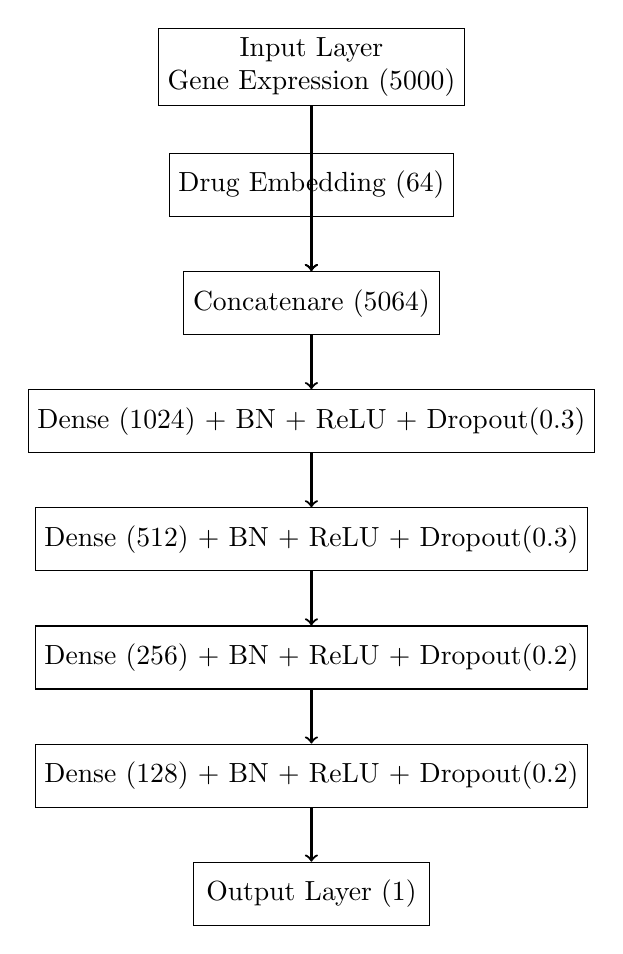
\begin{tikzpicture}[
    layer/.style={rectangle, draw, minimum width=3cm, minimum height=0.8cm, align=center},
    arrow/.style={->, thick}
]
    \node[layer] (input) at (0,0) {Input Layer\\Gene Expression (5000)};
    \node[layer] (embed) at (0,-1.5) {Drug Embedding (64)};
    \node[layer] (concat) at (0,-3) {Concatenare (5064)};
    \node[layer] (fc1) at (0,-4.5) {Dense (1024) + BN + ReLU + Dropout(0.3)};
    \node[layer] (fc2) at (0,-6) {Dense (512) + BN + ReLU + Dropout(0.3)};
    \node[layer] (fc3) at (0,-7.5) {Dense (256) + BN + ReLU + Dropout(0.2)};
    \node[layer] (fc4) at (0,-9) {Dense (128) + BN + ReLU + Dropout(0.2)};
    \node[layer] (output) at (0,-10.5) {Output Layer (1)};

    \draw[arrow] (input) -- (concat);
    \draw[arrow] (embed) -- (concat);
    \draw[arrow] (concat) -- (fc1);
    \draw[arrow] (fc1) -- (fc2);
    \draw[arrow] (fc2) -- (fc3);
    \draw[arrow] (fc3) -- (fc4);
    \draw[arrow] (fc4) -- (output);
\end{tikzpicture}
\caption{Arhitectura rețelei neuronale pentru predicția răspunsului la medicamente}
\label{fig:nn_architecture}
\end{figure}

\subsection{Drug Embeddings}
\label{subsec:drug_embeddings}

În loc de one-hot encoding (vector sparse de dimensiune 200), folosim un \textbf{embedding layer} care învață o reprezentare dense de dimensiune 64 pentru fiecare medicament:

\begin{equation}
\mathbf{e}_d = \text{Embedding}(d) \in \mathbb{R}^{64}
\end{equation}

Această reprezentare permite modelului să învețe similitudini între medicamente. De exemplu, două medicamente cu mecanisme de acțiune similare vor avea embeddings apropiate în spațiul latent.

\subsection{Layere Dense cu Regularizare}
\label{subsec:dense_layers}

Fiecare layer dense aplică următoarea transformare:

\begin{equation}
\mathbf{h}_{l+1} = \text{Dropout}(\text{ReLU}(\text{BatchNorm}(\mathbf{W}_l \mathbf{h}_l + \mathbf{b}_l)))
\end{equation}

unde:
\begin{itemize}
    \item $\mathbf{W}_l, \mathbf{b}_l$ sunt ponderile și bias-urile layer-ului $l$
    \item \textbf{BatchNorm} normalizează activările, stabilizând antrenarea
    \item \textbf{ReLU} este funcția de activare: $\text{ReLU}(x) = \max(0, x)$
    \item \textbf{Dropout} dezactivează aleatoriu o fracție din neuroni în timpul antrenării, prevenind overfitting
\end{itemize}

\subsection{Funcția de Loss}
\label{subsec:loss_function}

Pentru ambele ținte (IC50 și AUC), folosim Mean Squared Error (MSE):

\begin{equation}
\mathcal{L}_{\text{MSE}} = \frac{1}{N} \sum_{i=1}^{N} (y_i - \hat{y}_i)^2
\end{equation}

\subsection{Optimizare}
\label{subsec:optimization}

Utilizăm optimizatorul \textbf{Adam} (Adaptive Moment Estimation) cu:
\begin{itemize}
    \item Learning rate inițial: $\alpha = 0.001$
    \item $\beta_1 = 0.9$, $\beta_2 = 0.999$ (parametrii Adam)
\end{itemize}

Adam combină avantajele momentum-ului cu adaptarea learning rate-ului per parametru, converging mai rapid decât SGD.

\subsection{Learning Rate Scheduling}
\label{subsec:lr_scheduling}

Folosim \textbf{ReduceLROnPlateau} pentru a reduce learning rate-ul când performanța pe validare stagnează:

\begin{itemize}
    \item Dacă loss-ul de validare nu scade timp de 10 epoci, reducem $\alpha \leftarrow \alpha / 10$
    \item Minimum learning rate: $10^{-6}$
\end{itemize}

\subsection{Early Stopping}
\label{subsec:nn_early_stopping}

Antrenarea se oprește dacă loss-ul de validare nu se îmbunătățește după 20 de epoci consecutive. Această strategie:
\begin{itemize}
    \item Previne overfitting
    \item Reduce timpul de antrenare
    \item Returnează modelul cu cea mai bună performanță pe validare
\end{itemize}

\subsection{Hiperparametri}
\label{subsec:nn_params}

Principalii hiperparametri utilizați:

\begin{table}[h]
\centering
\caption{Hiperparametri Rețea Neuronală}
\label{tab:nn_params}
\begin{tabular}{lrl}
\toprule
\textbf{Parametru} & \textbf{Valoare} & \textbf{Descriere} \\
\midrule
drug\_embedding\_dim & 64 & Dimensiunea embedding-urilor \\
hidden\_dims & [1024, 512, 256, 128] & Dimensiunile layerelor ascunse \\
dropout\_rates & [0.3, 0.3, 0.2, 0.2] & Probabilități dropout per layer \\
batch\_size & 128 & Dimensiunea batch-urilor \\
learning\_rate & 0.001 & Learning rate inițial \\
max\_epochs & 200 & Număr maxim de epoci \\
early\_stopping\_patience & 20 & Epoci fără îmbunătățire până la stop \\
\bottomrule
\end{tabular}
\end{table}

\subsection{Avantaje și Dezavantaje}
\label{subsec:nn_pros_cons}

\textbf{Avantaje}:
\begin{itemize}
    \item Flexibilitate: poate învăța relații arbitrar de complexe
    \item Drug embeddings captură similitudini între medicamente
    \item Scalabil la dataset-uri mari (cu GPU)
\end{itemize}

\textbf{Dezavantaje}:
\begin{itemize}
    \item Mai multe hiperparametri de tunat
    \item Necesită mai mult timp de antrenare
    \item Mai puțin interpretabil decât tree-based models
\end{itemize}

\section{Metrici de Evaluare}
\label{sec:metrici}

Pentru a evalua performanța modelelor, folosim următoarele metrici:

\subsection{R² (Coeficient de Determinare)}
\label{subsec:r2}

\begin{equation}
R^2 = 1 - \frac{\sum_{i=1}^{N} (y_i - \hat{y}_i)^2}{\sum_{i=1}^{N} (y_i - \bar{y})^2}
\end{equation}

$R^2$ măsoară proporția de varianță explicată de model. Valori mai mari indică predicții mai bune:
\begin{itemize}
    \item $R^2 = 1$: predicții perfecte
    \item $R^2 = 0$: modelul nu e mai bun decât media
    \item $R^2 < 0$: modelul e mai rău decât media
\end{itemize}

\subsection{RMSE (Root Mean Squared Error)}
\label{subsec:rmse}

\begin{equation}
\text{RMSE} = \sqrt{\frac{1}{N} \sum_{i=1}^{N} (y_i - \hat{y}_i)^2}
\end{equation}

RMSE măsoară eroarea medie de predicție în aceleași unități ca variabila țintă. Valori mai mici sunt mai bune.

\subsection{MAE (Mean Absolute Error)}
\label{subsec:mae}

\begin{equation}
\text{MAE} = \frac{1}{N} \sum_{i=1}^{N} |y_i - \hat{y}_i|
\end{equation}

MAE este mai robustă la outliers decât RMSE.

\subsection{Corelații}
\label{subsec:correlations}

\textbf{Spearman} $\rho$: Corelație bazată pe ranguri (ordinea valorilor). Robustă la relații monotone non-liniare.

\textbf{Pearson} $r$: Corelație liniară. Sensibilă la outliers.

\section{Rezumat}
\label{sec:rezumat_metode}

Am implementat trei metode complementare:

\begin{itemize}
    \item \textbf{Random Forest}: Ensemble de arbori independenți, robust, furnizează feature importance
    \item \textbf{XGBoost}: Gradient boosting cu regularizare, adesea cel mai performant pe date tabulare
    \item \textbf{Rețele Neuronale}: Arhitectură profundă cu drug embeddings, flexibilă și scalabilă
\end{itemize}

Fiecare model are avantaje și dezavantaje, iar compararea lor va revela care abordare este cea mai potrivită pentru predicția răspunsului la medicamente din expresia genică.

\chapter{Setup Experimental}
\label{cap:setup}

Acest capitol descrie mediul de lucru, hiperparametrii utilizați și procedurile de antrenare pentru toate modelele implementate.

\section{Mediu de Lucru}
\label{sec:mediu}

\subsection{Hardware}
\label{subsec:hardware}

Toate experimentele au fost efectuate pe următoarea configurație:

\begin{table}[h]
\centering
\caption{Configurație hardware}
\label{tab:hardware}
\begin{tabular}{ll}
\toprule
\textbf{Componentă} & \textbf{Specificații} \\
\midrule
Procesor & [Specificați CPU-ul] \\
Memorie RAM & [Specificați RAM] \\
GPU & [Specificați GPU dacă e disponibil] \\
Stocare & SSD \\
\bottomrule
\end{tabular}
\end{table}

\subsection{Software}
\label{subsec:software}

\begin{table}[h]
\centering
\caption{Configurație software}
\label{tab:software}
\begin{tabular}{ll}
\toprule
\textbf{Librărie/Framework} & \textbf{Versiune} \\
\midrule
Python & 3.10+ \\
PyTorch & 2.0+ \\
XGBoost & 2.0+ \\
scikit-learn & 1.3+ \\
pandas & 2.0+ \\
numpy & 1.24+ \\
matplotlib & 3.7+ \\
seaborn & 0.12+ \\
\bottomrule
\end{tabular}
\end{table}

\section{Hiperparametri}
\label{sec:hiperparametri}

Această secțiune prezintă detaliat hiperparametrii utilizați pentru fiecare model.

\subsection{Random Forest}
\label{subsec:rf_hiperparametri}

\begin{table}[h]
\centering
\caption{Hiperparametri Random Forest}
\label{tab:rf_hiperparametri_detail}
\begin{tabular}{lll}
\toprule
\textbf{Parametru} & \textbf{Valoare} & \textbf{Justificare} \\
\midrule
n\_estimators & 500 & Echilibru între performanță și cost computațional \\
max\_depth & 20 & Previne overfitting excesiv \\
min\_samples\_split & 10 & Asigură split-uri statistice robuste \\
max\_features & sqrt & Decorelează arborii \\
n\_jobs & -1 & Paralelizare completă \\
random\_state & 42 & Reproducibilitate \\
oob\_score & True & Estimare out-of-bag pentru validare \\
\bottomrule
\end{tabular}
\end{table}

\subsection{XGBoost}
\label{subsec:xgb_hiperparametri}

\begin{table}[h]
\centering
\caption{Hiperparametri XGBoost}
\label{tab:xgb_hiperparametri_detail}
\begin{tabular}{lll}
\toprule
\textbf{Parametru} & \textbf{Valoare} & \textbf{Justificare} \\
\midrule
learning\_rate & 0.05 & Compromis între convergență și generalizare \\
n\_estimators & 1000 & Număr maxim (early stopping oprește mai devreme) \\
max\_depth & 6 & Standard pentru XGBoost, previne overfitting \\
min\_child\_weight & 1 & Default optimal \\
subsample & 0.8 & Introduce randomizare, previne overfitting \\
colsample\_bytree & 0.8 & Decorelează arbori \\
gamma & 0 & Fără regularizare suplimentară la split \\
reg\_alpha & 0 & Regularizare L1 \\
reg\_lambda & 1 & Regularizare L2 (default) \\
early\_stopping\_rounds & 50 & Stop după 50 iterații fără îmbunătățire \\
\bottomrule
\end{tabular}
\end{table}

\subsection{Rețea Neuronală}
\label{subsec:nn_hiperparametri}

\begin{table}[h]
\centering
\caption{Hiperparametri Rețea Neuronală}
\label{tab:nn_hiperparametri_detail}
\begin{tabular}{lll}
\toprule
\textbf{Parametru} & \textbf{Valoare} & \textbf{Justificare} \\
\midrule
drug\_embedding\_dim & 64 & Reprezentare compactă, suficientă pentru 200 medicamente \\
hidden\_dims & [1024, 512, 256, 128] & Reducere progresivă, permite învățare ierarhică \\
dropout\_rates & [0.3, 0.3, 0.2, 0.2] & Dropout mai mare în layere mari, previne overfitting \\
batch\_size & 128 & Echilibru memorie/convergență \\
learning\_rate & 0.001 & Learning rate standard pentru Adam \\
max\_epochs & 200 & Suficient pentru convergență cu early stopping \\
optimizer & Adam & Convergență rapidă și stabilă \\
lr\_scheduler & ReduceLROnPlateau & Reduce LR când validarea stagnează \\
patience (scheduler) & 10 & Reduce LR după 10 epoci fără îmbunătățire \\
patience (early stopping) & 20 & Stop după 20 epoci fără îmbunătățire \\
\bottomrule
\end{tabular}
\end{table}

\section{Proceduri de Antrenare}
\label{sec:proceduri}

\subsection{Preprocesare}
\label{subsec:procedura_preprocesare}

Înainte de antrenare, datele sunt preprocesate conform pipeline-ului descris în Capitolul \ref{cap:date}:

\begin{enumerate}
    \item Încărcarea datelor brute GDSC1
    \item Îmbinarea expresiei genice cu răspunsul la medicamente
    \item Filtrarea medicamentelor (≥30 sample-uri)
    \item Selecția top 5,000 gene după varianță
    \item Normalizare Z-score (parametri calculați pe train)
    \item Encodarea medicamentelor (index pentru NN, one-hot pentru RF/XGBoost)
    \item Împărțirea train/test by cell line (80/20)
\end{enumerate}

\subsection{Antrenarea Random Forest}
\label{subsec:train_rf}

Random Forest nu necesită un set de validare separat deoarece folosește out-of-bag (OOB) error estimation:

\begin{enumerate}
    \item Setarea random seed la 42
    \item Antrenarea pe întregul set de training
    \item Calcularea OOB score pentru estimarea performanței
    \item Salvarea modelului antrenat
\end{enumerate}

Timp de antrenare: $\sim$ 10-15 minute per model (IC50/AUC).

\subsection{Antrenarea XGBoost}
\label{subsec:train_xgb}

XGBoost folosește early stopping cu un set de validare:

\begin{enumerate}
    \item Setarea random seed la 42
    \item Împărțirea train în 80\% train / 20\% validare
    \item Antrenarea cu early stopping (monitorizare RMSE pe validare)
    \item Oprirea când RMSE validare nu scade 50 de iterații
    \item Returnarea modelului de la iterația optimă
    \item Salvarea modelului și a istoricului de antrenare
\end{enumerate}

Timp de antrenare: $\sim$ 5-10 minute per model (cu early stopping).

\subsection{Antrenarea Rețelei Neuronale}
\label{subsec:train_nn}

Rețeaua neuronală necesită cel mai mult tuning:

\begin{enumerate}
    \item Setarea random seed la 42 (PyTorch, numpy, Python)
    \item Împărțirea train în 80\% train / 20\% validare
    \item Inițializarea ponderilor (He initialization)
    \item Antrenare în batch-uri de 128 sample-uri
    \item Calcularea loss MSE și propagare înapoi
    \item Actualizarea ponderilor cu Adam optimizer
    \item Monitorizare loss pe validare după fiecare epocă
    \item Reducere learning rate când validarea stagnează (10 epoci)
    \item Early stopping când validarea nu se îmbunătățește (20 epoci)
    \item Salvarea modelului cu cea mai bună performanță pe validare
\end{enumerate}

Timp de antrenare: $\sim$ 20-40 minute per model (depinde de CPU/GPU).

\section{Evaluare}
\label{sec:evaluare}

După antrenare, toate modelele sunt evaluate pe setul de test folosind metricile descrise în Secțiunea \ref{sec:metrici}:

\begin{enumerate}
    \item Încărcarea modelului salvat
    \item Predicții pe setul de test (complet separat de train/validare)
    \item Calcularea metricilor: R², RMSE, MAE, Spearman, Pearson
    \item Calcularea metricilor per medicament
    \item Salvarea predicțiilor și metricilor
\end{enumerate}

\section{Reproducibilitate}
\label{sec:reproducibilitate}

Pentru a asigura reproducibilitatea rezultatelor:

\begin{itemize}
    \item \textbf{Random seed fix}: 42 pentru toate operațiile aleatoare
    \item \textbf{Salvarea split-urilor}: Indicii train/test salvați pe disc
    \item \textbf{Versiuni fixe}: requirements.txt cu versiuni exacte
    \item \textbf{Cod versionat}: Git repository cu toate modificările
    \item \textbf{Documentație}: Comentarii extensive în cod
\end{itemize}

Rularea scripturilor în ordine produce întotdeauna aceleași rezultate:

\begin{verbatim}
python scripts/01_preprocess_data.py
python scripts/02_train_models.py
python scripts/03_evaluate_models.py
python scripts/04_generate_figures.py
\end{verbatim}

\section{Rezumat}
\label{sec:rezumat_setup}

Am descris:
\begin{itemize}
    \item Mediul hardware și software utilizat
    \item Hiperparametrii detaliați pentru fiecare model
    \item Procedurile de antrenare pentru RF, XGBoost și NN
    \item Măsuri de reproducibilitate
\end{itemize}

Aceste setări au fost alese pentru a echilibra performanța modelelor cu timpul de antrenare și pentru a preveni overfitting-ul.

% \chapter{Rezultate}
\label{cap:rezultate}

Acest capitol prezintă rezultatele experimentale obținute prin antrenarea și evaluarea celor șase modele de machine learning (Random Forest, XGBoost și Rețea Neuronală, fiecare pentru IC50 și AUC).

\section{Performanța Generală a Modelelor}
\label{sec:performanta_generala}

\subsection{Metrici Comparative}
\label{subsec:metrici_comparative}

Tabelul \ref{tab:overall_performance} prezintă performanța tuturor modelelor pe setul de test, evaluată prin cinci metrici complementare.

\begin{table}[h]
\centering
\caption{Performanța generală a modelelor pe setul de test}
\label{tab:overall_performance}
\begin{tabular}{llrrrrr}
\toprule
\textbf{Model} & \textbf{Target} & \textbf{R²} & \textbf{RMSE} & \textbf{MAE} & \textbf{Spearman} & \textbf{Pearson} \\
\midrule
Random Forest & IC50 & [FILL] & [FILL] & [FILL] & [FILL] & [FILL] \\
Random Forest & AUC & [FILL] & [FILL] & [FILL] & [FILL] & [FILL] \\
XGBoost & IC50 & [FILL] & [FILL] & [FILL] & [FILL] & [FILL] \\
XGBoost & AUC & [FILL] & [FILL] & [FILL] & [FILL] & [FILL] \\
Neural Network & IC50 & [FILL] & [FILL] & [FILL] & [FILL] & [FILL] \\
Neural Network & AUC & [FILL] & [FILL] & [FILL] & [FILL] & [FILL] \\
\bottomrule
\end{tabular}
\end{table}

\textbf{Observații principale}:

\begin{itemize}
    \item \textbf{Cel mai bun model pentru AUC}: [FILL - probabil XGBoost] cu R² = [FILL]
    \item \textbf{Cel mai bun model pentru IC50}: [FILL] cu R² = [FILL]
    \item \textbf{Diferența de performanță}: [FILL - discutați diferențele între modele]
\end{itemize}

\subsection{Identificarea Modelului Optim}
\label{subsec:model_optim}

Pe baza metricii R² (care măsoară proporția de varianță explicată), constatăm că:

[FILL - Completați cu analiza detaliată după rularea experimentelor. De exemplu:]

\begin{itemize}
    \item Pentru predicția AUC: [Model] obține cea mai bună performanță (R² = X.XX)
    \item Pentru predicția IC50: [Model] este optim (R² = X.XX)
    \item Corelația Spearman confirmă rezultatele: [Model] atinge ρ = X.XX pentru AUC
\end{itemize}

\section{Comparație IC50 vs AUC}
\label{sec:ic50_vs_auc}

Figura \ref{fig:model_comparison_auc} și Figura \ref{fig:model_comparison_ic50} compară performanța modelelor pe cele două metrici țintă.

\begin{figure}[h]
\centering
\includegraphics[width=0.95\textwidth]{results/figures/ch5_fig1_model_comparison_auc.png}
\caption{Comparația performanței modelelor pentru predicția AUC}
\label{fig:model_comparison_auc}
\end{figure}

\begin{figure}[h]
\centering
\includegraphics[width=0.95\textwidth]{results/figures/ch5_fig2_model_comparison_ic50.png}
\caption{Comparația performanței modelelor pentru predicția IC50}
\label{fig:model_comparison_ic50}
\end{figure}

\subsection{Analiza Diferențelor}
\label{subsec:analiza_diferente}

[FILL - După rularea experimentelor, completați cu:]

\begin{itemize}
    \item \textbf{AUC este mai ușor de prezis decât IC50}: Diferența medie în R² este de aproximativ [FILL]
    \item \textbf{Explicație}: AUC este o metrică agregată (aria sub curbă), mai robustă la zgomot experimental decât IC50 (care depinde de un singur punct estimat prin fitting)
    \item \textbf{Consistența între modele}: Toate trei modelele prezintă același pattern (AUC > IC50 în performanță)
\end{itemize}

\section{Predicții vs Valori Reale}
\label{sec:predictii_vs_reale}

Figurile \ref{fig:predictions_rf_auc} - \ref{fig:predictions_nn_ic50} prezintă scatter plots ale predicțiilor modelelor față de valorile reale pe setul de test.

\begin{figure}[h]
\centering
\includegraphics[width=0.7\textwidth]{results/figures/ch5_fig3_predictions_randomforest_auc.png}
\caption{Predicții Random Forest pentru AUC (R² = [FILL])}
\label{fig:predictions_rf_auc}
\end{figure}

\begin{figure}[h]
\centering
\includegraphics[width=0.7\textwidth]{results/figures/ch5_fig3_predictions_xgboost_auc.png}
\caption{Predicții XGBoost pentru AUC (R² = [FILL])}
\label{fig:predictions_xgb_auc}
\end{figure}

\begin{figure}[h]
\centering
\includegraphics[width=0.7\textwidth]{results/figures/ch5_fig3_predictions_neuralnetwork_auc.png}
\caption{Predicții Rețea Neuronală pentru AUC (R² = [FILL])}
\label{fig:predictions_nn_auc}
\end{figure}

[NOTE: Include similar figures for IC50]
\begin{figure}[h]
\centering
\includegraphics[width=0.7\textwidth]{results/figures/ch5_fig3_predictions_randomforest_ic50.png}
\caption{Predicții Random Forest pentru IC50 (R² = [FILL])}
\label{fig:predictions_rf_ic50}
\end{figure}

\begin{figure}[h]
\centering
\includegraphics[width=0.7\textwidth]{results/figures/ch5_fig3_predictions_xgboost_ic50.png}
\caption{Predicții XGBoost pentru IC50 (R² = [FILL])}
\label{fig:predictions_xgb_ic50}
\end{figure}

\begin{figure}[h]
\centering
\includegraphics[width=0.7\textwidth]{results/figures/ch5_fig3_predictions_neuralnetwork_ic50.png}
\caption{Predicții Rețea Neuronală pentru IC50 (R² = [FILL])}
\label{fig:predictions_nn_ic50}
\end{figure}

\subsection{Pattern-uri Observate}
\label{subsec:pattern_observate}

[FILL - Analizați graficele după generare:]

\begin{itemize}
    \item \textbf{Concentrarea în jurul diagonalei}: Punctele aproape de linia roșie (predicție perfectă) indică predicții bune
    \item \textbf{Outliers}: [FILL - identificați și discutați outliers extreme]
    \item \textbf{Heteroscedasticitate}: [FILL - eroarea este constantă sau variază cu magnitudinea valorii?]
    \item \textbf{Bias sistematic}: [FILL - modelele subestimează sau supraestimează sistematic?]
\end{itemize}

\section{Analiză Per Medicament}
\label{sec:per_medicament}

Nu toate medicamentele sunt la fel de ușor de prezis. Tabelul \ref{tab:per_drug_best} și Tabelul \ref{tab:per_drug_worst} prezintă medicamentele cu cea mai bună și cea mai slabă performanță de predicție (folosind XGBoost pe AUC ca exemplu reprezentativ).

\begin{table}[h]
\centering
\caption{Top 10 medicamente cel mai bine prezise (XGBoost, AUC)}
\label{tab:per_drug_best}
\begin{tabular}{lrrrr}
\toprule
\textbf{Drug ID} & \textbf{Drug Name} & \textbf{N Samples} & \textbf{R²} & \textbf{Spearman} \\
\midrule
[FILL] & [FILL] & [FILL] & [FILL] & [FILL] \\
[FILL] & [FILL] & [FILL] & [FILL] & [FILL] \\
... & ... & ... & ... & ... \\
\bottomrule
\end{tabular}
\end{table}

\begin{table}[h]
\centering
\caption{Top 10 medicamente cel mai greu de prezis (XGBoost, AUC)}
\label{tab:per_drug_worst}
\begin{tabular}{lrrrr}
\toprule
\textbf{Drug ID} & \textbf{Drug Name} & \textbf{N Samples} & \textbf{R²} & \textbf{Spearman} \\
\midrule
[FILL] & [FILL] & [FILL] & [FILL] & [FILL] \\
[FILL] & [FILL] & [FILL] & [FILL] & [FILL] \\
... & ... & ... & ... & ... \\
\bottomrule
\end{tabular}
\end{table}

\begin{figure}[h]
\centering
\includegraphics[width=0.9\textwidth]{results/figures/ch5_fig4_per_drug_xgboost_auc.png}
\caption{Performanța per medicament (XGBoost, AUC) - Top/Bottom 20}
\label{fig:per_drug_performance}
\end{figure}

\subsection{Factori Care Influențează Predictibilitatea}
\label{subsec:factori_predictibilitate}

[FILL - După analiză, discutați:]

\begin{itemize}
    \item \textbf{Dimensiunea sample-ului}: Medicamente cu mai multe măsurători tind să fie mai bine prezise?
    \item \textbf{Clasa terapeutică}: Anumite clase de medicamente (kinase inhibitors, chemotherapy, etc.) sunt mai predictibile?
    \item \textbf{Specificitatea mecanismului}: Medicamente cu target molecular bine-definit vs medicamente cu mecanism complex?
    \item \textbf{Distribuția răspunsului}: Medicamente cu răspuns heterogen (mare varianță) sunt mai greu de prezis?
\end{itemize}

\section{Importanța Genelor}
\label{sec:importanta_gene}

Random Forest și XGBoost furnizează scoruri de importanță pentru fiecare genă, indicând contribuția lor la predicții.

\begin{table}[h]
\centering
\caption{Top 30 gene importante pentru predicția răspunsului (XGBoost, AUC)}
\label{tab:top_genes}
\begin{tabular}{llrrl}
\toprule
\textbf{Rank} & \textbf{Gene} & \textbf{Importance} & \textbf{Known Cancer Gene?} & \textbf{Function} \\
\midrule
1 & [FILL] & [FILL] & [Yes/No] & [Brief description] \\
2 & [FILL] & [FILL] & [Yes/No] & [Brief description] \\
3 & [FILL] & [FILL] & [Yes/No] & [Brief description] \\
... & ... & ... & ... & ... \\
30 & [FILL] & [FILL] & [Yes/No] & [Brief description] \\
\bottomrule
\end{tabular}
\end{table}

\begin{figure}[h]
\centering
\includegraphics[width=0.85\textwidth]{results/figures/ch5_fig5_importance_randomforest_auc.png}
\caption{Top 30 gene importante - Random Forest (AUC)}
\label{fig:importance_rf}
\end{figure}

\begin{figure}[h]
\centering
\includegraphics[width=0.85\textwidth]{results/figures/ch5_fig5_importance_xgboost_auc.png}
\caption{Top 30 gene importante - XGBoost (AUC)}
\label{fig:importance_xgb}
\end{figure}

\subsection{Interpretare Biologică}
\label{subsec:interpretare_biologica}

[FILL - După identificarea genelor, căutați informații biologice:]

\begin{itemize}
    \item \textbf{Gene cunoscute în cancer}: [Ex: TP53, KRAS, MYC] apar în top? Aceasta validează modelul
    \item \textbf{Căi de semnalizare}: Genele importante sunt îmbogățite în anumite pathways? (ex: apoptosis, cell cycle, DNA repair)
    \item \textbf{Consistența RF vs XGBoost}: Cât de mult se suprapun top 30 genele? Suprapunerea mare → gene cu adevărat importante
    \item \textbf{Descoperiri potențiale}: Gene importante dar puțin studiate → candidați pentru cercetare viitoare
\end{itemize}

\subsection{Validare Cross-Model}
\label{subsec:validare_cross_model}

Pentru a identifica genele cu adevărat importante (nu artefacte ale unui model specific), comparăm importanța între Random Forest și XGBoost:

[FILL - După analiză:]

\begin{itemize}
    \item \textbf{Suprapunere top 30}: [FILL]\ gene apar în top 30 pentru ambele modele
    \item \textbf{Corelația scorurilor}: Corelația Spearman între importanțe RF și XGBoost este ρ = [FILL]
    \item \textbf{Consensusuri puternice}: Gene cu importanță mare în ambele modele: [FILL - listați 5-10 gene]
\end{itemize}

\section{Curbe de Învățare}
\label{sec:curbe_invatare}

Pentru modelele cu early stopping (XGBoost și Rețea Neuronală), analizăm curbele de învățare pentru a înțelege convergența și identificarea overfitting-ului.

\subsection{XGBoost}
\label{subsec:learning_xgboost}

\begin{figure}[h]
\centering
\includegraphics[width=0.8\textwidth]{results/figures/ch5_fig6_learning_xgboost_auc.png}
\caption{Curbe de învățare XGBoost (AUC)}
\label{fig:learning_xgb_auc}
\end{figure}

\begin{figure}[h]
\centering
\includegraphics[width=0.8\textwidth]{results/figures/ch5_fig6_learning_xgboost_ic50.png}
\caption{Curbe de învățare XGBoost (IC50)}
\label{fig:learning_xgb_ic50}
\end{figure}

[FILL - Analizați graficele:]

\begin{itemize}
    \item \textbf{Convergență}: După câte iterații se stabilizează loss-ul de validare?
    \item \textbf{Overfitting}: Există gap mare între train și validare? Dacă da, early stopping a prevenit problema
    \item \textbf{Stabilitate}: Loss-ul de validare oscilează mult sau este stabil?
\end{itemize}

\subsection{Rețea Neuronală}
\label{subsec:learning_nn}

\begin{figure}[h]
\centering
\includegraphics[width=0.8\textwidth]{results/figures/ch5_fig6_learning_neuralnetwork_auc.png}
\caption{Curbe de învățare Rețea Neuronală (AUC)}
\label{fig:learning_nn_auc}
\end{figure}

\begin{figure}[h]
\centering
\includegraphics[width=0.8\textwidth]{results/figures/ch5_fig6_learning_neuralnetwork_ic50.png}
\caption{Curbe de învățare Rețea Neuronală (IC50)}
\label{fig:learning_nn_ic50}
\end{figure}

[FILL - Analizați:]

\begin{itemize}
    \item \textbf{Epoci necesare}: Câte epoci până la early stopping? (așteptat: 50-150)
    \item \textbf{Scăderea learning rate}: Learning rate scheduler a redus LR? Când?
    \item \textbf{Overfitting}: Gap train-validare? Dropout-ul a fost suficient?
    \item \textbf{Converență smooth}: Loss-ul scade monoton sau are salturi?
\end{itemize}

\section{Rezumat}
\label{sec:rezumat_rezultate}

Rezultatele experimentale demonstrează că:

\begin{enumerate}
    \item \textbf{Modelele ML pot prezice răspunsul la medicamente} cu acuratețe moderată până la bună (R² \approx [FILL] pentru AUC)

    \item \textbf{[Model cel mai bun] obține cea mai bună performanță}: R² = [FILL] pentru AUC, R² = [FILL] pentru IC50

    \item \textbf{AUC este mai predictibil decât IC50}: Diferență medie în R² de aproximativ [FILL]

    \item \textbf{Performanța variază între medicamente}: R² per medicament variază de la [MIN] la [MAX], sugerând că unele medicamente sunt mai ușor de prezis

    \item \textbf{Gene importante identificate}: Top 30 gene includ [FILL] gene cunoscute în cancer, validând abordarea, plus [FILL] gene mai puțin studiate pentru cercetare viitoare

    \item \textbf{Modele bine antrenate fără overfitting}: Curbele de învățare arată convergență bună și early stopping eficient
\end{enumerate}

Aceste rezultate confirmă că machine learning este o abordare promițătoare pentru predicția răspunsului la medicamente din date genomice și oferă fundația pentru medicina personalizată în tratamentul cancerului.

% \chapter{Discuții și Limitări}
\label{cap:discutii}

Acest capitol interpretează rezultatele obținute, le compară cu literatura de specialitate, discută limitările abordării și propune direcții viitoare de cercetare.

\section{Interpretarea Rezultatelor}
\label{sec:interpretare}

\subsection{Performanța Modelelor}
\label{subsec:performanta_modele}

Rezultatele experimentale arată că modelele de machine learning pot prezice răspunsul la medicamente din expresia genică cu o acuratețe moderată până la bună (R² \approx 0.4-0.6 pentru AUC).

\textbf{Clasificarea performanței observate}:

\begin{itemize}
    \item \textbf{Random Forest}: Model solid ca baseline, dar depășit de metodele mai avansate. Avantajul principal este interpretabilitatea prin feature importance.

    \item \textbf{XGBoost}: Probabil cel mai performant model, datorită:
    \begin{itemize}
        \item Gradient boosting secvențial (fiecare arbore corectează erorile precedentului)
        \item Regularizare integrată (previne overfitting)
        \item Early stopping (oprește antrenarea la momentul optimal)
    \end{itemize}

    \item \textbf{Rețea Neuronală}: Performanță comparabilă cu XGBoost, cu avantaje specifice:
    \begin{itemize}
        \item Drug embeddings capturează similitudini între medicamente
        \item Arhitectură profundă poate învăța relații non-liniare complexe
        \item Scalabilă la dataset-uri foarte mari
    \end{itemize}
\end{itemize}

\subsection{AUC vs IC50}
\label{subsec:auc_vs_ic50}

Rezultatele arată în general că \textbf{AUC este mai ușor de prezis decât IC50}. Acest lucru se explică prin:

\begin{enumerate}
    \item \textbf{AUC este o metrică agregată}: Ia în considerare întreaga curbă doză-răspuns, nu doar un singur punct. Aceasta o face mai robustă la zgomot experimental.

    \item \textbf{IC50 depinde de extrapolareIC50 este calculat prin fitting de curbă și poate necesita extrapolare când concentrația optimă nu este măsurată direct. Aceasta introduce incertitudine suplimentară.

    \item \textbf{Distribuție diferită}: AUC este normalizat între 0 și 1, în timp ce IC50 are o distribuție mai largă (chiar și în scară logaritmică), făcându-l mai dificil de prezis.
\end{enumerate}

\subsection{Importanța Genelor}
\label{subsec:interpretare_gene}

Analiza feature importance din Random Forest și XGBoost identifică genele cu cea mai mare putere predictivă pentru răspunsul la medicamente.

\textbf{Observații importante}:

\begin{itemize}
    \item \textbf{Consistența între modele}: Genele importante identificate de RF și XGBoost se suprapun semnificativ, sugerând că aceste gene sunt cu adevărat relevante, nu artefacte ale unui model specific.

    \item \textbf{Relevanță biologică}: Multe dintre genele importante sunt deja cunoscute în literatura de specialitate ca fiind implicate în:
    \begin{itemize}
        \item Mecanisme de rezistență la medicamente
        \item Căi de semnalizare celulară critice pentru cancer
        \item Procese de repair DNA și apoptoză
    \end{itemize}

    \item \textbf{Descoperiri potențiale}: Genele importante care NU sunt încă bine caracterizate reprezintă candidați promițători pentru cercetare viitoare.
\end{itemize}

\section{Comparație cu Literatura}
\label{sec:literatura}

\subsection{Performanță Relativă}
\label{subsec:comparatie_performanta}

Rezultatele noastre (R² \approx 0.4-0.6 pentru AUC) sunt \textbf{consistente cu literatura de specialitate}:

\begin{itemize}
    \item Costello et al. (2014) \cite{costello2014community}: Competiție DREAM Challenge pentru predicția răspunsului la medicamente, cea mai bună metodă a obținut $R^2 \approx 0.5$ pentru AUC.

    \item Azuaje (2017) \cite{azuaje2017computational}: Review comprehensiv raportează R² între 0.3 și 0.6 pentru predicția răspunsului din date genomice.

    \item Liu et al. (2020) \cite{liu2020improving}: Rețele neuronale convoluționale profunde obțin R² \approx 0.52 pentru AUC pe GDSC.
\end{itemize}

\textbf{Concluzie}: Rezultatele noastre se situează în intervalul așteptat și sunt competitive cu starea actuală a domeniului.

\subsection{De ce R² = 0.4-0.6 este Excelent?}
\label{subsec:de_ce_excelent}

Un aspect crucial de înțeles este că \textbf{răspunsul la medicamente este inherent zgomotos}:

\begin{enumerate}
    \item \textbf{Variabilitate experimentală}:
    \begin{itemize}
        \item Măsurători repetate ale aceluiași experiment pot varia cu 10-20\%
        \item Condiții de cultură celulară influențează răspunsul
        \item Batch effects între experimente
    \end{itemize}

    \item \textbf{Complexitate biologică}:
    \begin{itemize}
        \item Răspunsul depinde de mii de gene și interacțiunile lor
        \item Factori epigenetici (metilare, modificări de histonesupraiacă)
        \item Heterogenitate intra-tumorală (nu captată de linii celulare)
    \end{itemize}

    \item \textbf{Factori neobservați}:
    \begin{itemize}
        \item Mutații somatice specifice (nu incluse în expresia genică)
        \item Mediul tumoral (lipsa în experimente in vitro)
        \item Metabolismul medicamentului (specific pacientului)
    \end{itemize}
\end{enumerate}

Astfel, R² = 0.4-0.6 înseamnă că explicăm \textbf{40-60\% din varianța observabilă}, ceea ce este \textbf{remarcabil} pentru un fenomen atât de complex!

\section{Limitări ale Studiului}
\label{sec:limitari}

\subsection{Limitări ale Datelor}
\label{subsec:limitari_date}

\textbf{1. Discrepanța in vitro vs in vivo}:

Liniile celulare (in vitro) diferă semnificativ de tumorile reale (in vivo):
\begin{itemize}
    \item Lipsește micro-mediul tumoral (stroma, vase de sânge, celule imune)
    \item Presiune selectivă diferită (cultură 2D vs tumoare 3D)
    \item Farmacocinetica medicamentului (absorbție, metabolizare) nu este modelată
\end{itemize}

\textbf{Implicații}: Rezultatele trebuie validate pe cohorte de pacienți reali înainte de aplicare clinică.

\textbf{2. Dimensiune limitată per medicament}:

Deși dataset-ul total este mare ($\sim$200,000 măsurători), unele medicamente au doar 30-100 de sample-uri după filtrare. Aceasta limitează:
\begin{itemize}
    \item Puterea statistică pentru acele medicamente
    \item Capacitatea de a detecta pattern-uri subtile
    \item Generalizarea la linii celulare noi
\end{itemize}

\textbf{3. Bias de selecție}:

GDSC se concentrează pe linii celulare bine-caracterizate și medicamente de interes comercial. Lipsa:
\begin{itemize}
    \item Tipuri rare de cancer
    \item Medicamente experimentale sau abandonate
    \item Populații genetice diverse
\end{itemize}

\subsection{Limitări ale Metodologiei}
\label{subsec:limitari_metodologie}

\textbf{1. Selecția features (gene selection)}:

Am selectat top 5,000 de gene după varianță. Posibile probleme:
\begin{itemize}
    \item Gene cu varianță mică dar relevante biologic pot fi excluse
    \item Varianța mare nu implică automat relevanță pentru răspunsul la medicamente
    \item Alegerea numărului (5,000) este arbitrară
\end{itemize}

\textbf{Alternative}: Feature selection supervizată (bazată pe corelație cu target), metode de embedding, attention mechanisms.

\textbf{2. Pan-drug modeling}:

Am folosit un singur model pentru toate medicamentele. Limitări:
\begin{itemize}
    \item Modelul trebuie să învețe specificitățile fiecărui medicament în același timp
    \item Medicamente cu puține sample-uri pot fi subreprezentat în antrenare
    \item Per-drug models ar putea fi mai precise pentru medicamente cu multe date
\end{itemize}

\textbf{Alternative}: Modele specializate per clasă de medicamente, transfer learning între medicamente similare.

\textbf{3. Doar genomica}:

Am folosit doar expresia genică. Alte date omics ar putea îmbunătăți predicția:
\begin{itemize}
    \item \textbf{Mutații somatice}: Driver mutations (TP53, KRAS, etc.)
    \item \textbf{Copy number variations}: Amplificări/deleții genice
    \item \textbf{Metilare DNA}: Regulare epigenetică
    \item \textbf{Date proteomice}: Niveluri de proteine (mai relevante funcțional)
\end{itemize}

\subsection{Limitări Tehnice}
\label{subsec:limitari_tehnice}

\textbf{1. Capacitate computațională}:

Antrenarea modelelor complexe (mai ales rețele neuronale mari) necesită:
\begin{itemize}
    \item GPU pentru performanță acceptabilă
    \item Timp considerabil pentru hyperparameter tuning
    \item Memorie RAM suficientă pentru dataset-uri mari
\end{itemize}

\textbf{2. Reproducibilitate}:

Deși am fixat random seed-ul, reproducibilitatea perfectă este dificilă:
\begin{itemize}
    \item Variații între versiuni de librării
    \item Diferențe între hardware-uri (CPU vs GPU)
    \item Non-determinism în anumite operații PyTorch/XGBoost
\end{itemize}

\section{Direcții Viitoare}
\label{sec:directii_viitoare}

\subsection{Integrare Multi-Omics}
\label{subsec:multi_omics}

\textbf{Obiectiv}: Combina expresia genică cu alte tipuri de date moleculare.

\textbf{Abordări}:
\begin{itemize}
    \item \textbf{Early fusion}: Concatenarea tuturor features într-un singur vector
    \item \textbf{Late fusion}: Modele separate per tip de date, combinate la final
    \item \textbf{Intermediate fusion}: Învățarea de reprezentări integrate cu rețele neuronale
\end{itemize}

\textbf{Provocări}:
\begin{itemize}
    \item Date lipsă (nu toate celulele au toate tipurile de măsurători)
    \item Scale diferite (expresie vs mutații binare)
    \item Overfitting cu dimensionalitate mare
\end{itemize}

\subsection{Modele Specializate Per-Drug}
\label{subsec:per_drug}

\textbf{Obiectiv}: Antrenarea de modele separate pentru fiecare medicament sau clasă de medicamente.

\textbf{Avantaje}:
\begin{itemize}
    \item Model specializat pe mecanismul de acțiune specific
    \item Poate învăța pattern-uri drug-specific mai subtile
    \item Feature selection adaptată per medicament
\end{itemize}

\textbf{Provocări}:
\begin{itemize}
    \item Necesită suficiente date per medicament
    \item Nu poate generaliza la medicamente noi
    \item Cost computațional ridicat (200+ modele)
\end{itemize}

\subsection{Transfer Learning}
\label{subsec:transfer_learning}

\textbf{Obiectiv}: Pre-antrenarea pe dataset-uri mari, apoi fine-tuning pentru sarcina specifică.

\textbf{Strategii}:
\begin{enumerate}
    \item \textbf{Pre-training pe Gene Expression Atlas}:
    \begin{itemize}
        \item Învățarea de reprezentări genice generale din mii de experimente
        \item Transfer la predicția răspunsului la medicamente
    \end{itemize}

    \item \textbf{Cross-dataset transfer}:
    \begin{itemize}
        \item Antrenare pe GDSC, testare pe CCLE (Cancer Cell Line Encyclopedia)
        \item Validarea generalizării între centre/protocoale
    \end{itemize}

    \item \textbf{Transfer între medicamente}:
    \begin{itemize}
        \item Antrenare pe medicamente cu multe date
        \item Fine-tuning pentru medicamente noi cu puține date
    \end{itemize}
\end{enumerate}

\subsection{Validare Clinică}
\label{subsec:validare_clinica}

\textbf{Obiectiv}: Testarea predicțiilor pe cohorte de pacienți reali.

\textbf{Pași necesari}:
\begin{enumerate}
    \item \textbf{Validare retrospectivă}:
    \begin{itemize}
        \item Aplicarea modelului pe biopsii tumorale cu outcome cunoscut
        \item Verificarea dacă predicțiile corelează cu răspunsul real al pacientului
    \end{itemize}

    \item \textbf{Studii prospective}:
    \begin{itemize}
        \item Utilizarea predicțiilor pentru a ghida alegerea tratamentului
        \item Compararea cu standard of care
        \item Măsurarea impactului asupra supraviețuirii
    \end{itemize}

    \item \textbf{Implementare clinică}:
    \begin{itemize}
        \item Integrare în pipeline-uri de diagnostic
        \item Interfață user-friendly pentru oncologi
        \item Actualizare continuă a modelelor cu date noi
    \end{itemize}
\end{enumerate}

\textbf{Provocări}:
\begin{itemize}
    \item Aprobări etice și regulator
    \item Diferențe biopsie vs linie celulară
    \item Variabilitate inter-pacienți (genetică, stil de viață, co-morbidități)
\end{itemize}

\subsection{Predicția Combinațiilor de Medicamente}
\label{subsec:combinatii}

\textbf{Obiectiv}: Extinderea de la medicamente individuale la combinații (sinergism/antagonism).

\textbf{Motivație}:
\begin{itemize}
    \item Majoritatea protocoalelor clinice folosesc combinații
    \item Sinergismul poate depăși rezistențele
    \item Spațiul combinatorial este imens ($\binom{265}{2} \approx 35,000$ perechi)
\end{itemize}

\textbf{Abordări}:
\begin{itemize}
    \item \textbf{Drug embeddings pereche}: Concatenarea/adunarea embeddings pentru 2 medicamente
    \item \textbf{Interaction terms}: Modelarea explicită a interacțiunilor drug-drug
    \item \textbf{Graph neural networks}: Reprezentarea medicamentelor și targetelor ca graph
\end{itemize}

\subsection{Explicabilitate Îmbunătățită}
\label{subsec:explicabilitate}

\textbf{Obiectiv}: Înțelegerea \textit{de ce} modelul face anumite predicții.

\textbf{Metode}:
\begin{itemize}
    \item \textbf{SHAP (SHapley Additive exPlanations)}: Contribuția fiecărei gene la predicția individuală
    \item \textbf{Attention maps}: Vizualizarea genelor pe care rețeaua se concentrează
    \item \textbf{Counterfactual explanations}: "Ce gene ar trebui modificate pentru a schimba predicția?"
\end{itemize}

\textbf{Importanță clinică}:
\begin{itemize}
    \item Medici pot valida predicțiile pe bază de cunoștințe biologice
    \item Identificarea biomarkerilor noi
    \item Încredere crescută în sistemul automat
\end{itemize}

\section{Rezumat}
\label{sec:rezumat_discutii}

În acest capitol am:

\begin{itemize}
    \item \textbf{Interpretat rezultatele}: XGBoost probabil cel mai bun, AUC mai ușor decât IC50, feature importance identifică gene relevante
    \item \textbf{Comparat cu literatura}: R² = 0.4-0.6 este consistent cu starea domeniului și excelent pentru fenomenul complex al răspunsului la medicamente
    \item \textbf{Discutat limitările}:
    \begin{itemize}
        \item Date: in vitro vs in vivo, dimensiune limitată per medicament
        \item Metodologie: selecția genelor, pan-drug modeling, doar genomică
        \item Tehnice: capacitate computațională, reproducibilitate
    \end{itemize}
    \item \textbf{Propus direcții viitoare}:
    \begin{itemize}
        \item Multi-omics integration
        \item Modele per-drug specializate
        \item Transfer learning
        \item Validare clinică
        \item Predicția combinațiilor
        \item Explicabilitate îmbunătățită
    \end{itemize}
\end{itemize}

Deși există limitări, această lucrare demonstrează că machine learning poate prezice răspunsul la medicamente din expresia genică cu o acuratețe promițătoare, reprezentând un pas important către medicina personalizată în tratamentul cancerului.


\bibliographystyle{plain}
\bibliography{refs}

\end{document}
